\documentclass[../presentation.tex]{subfiles} % Parent file
\graphicspath{{\subfix{../images/}}} % Images path

\usetikzlibrary{positioning,3d}

\begin{document}

\section{Classification}

\begin{frame}

    \frametitle{AlexNet}
    \begin{tikzpicture}[scale=0.6, 3d view={120}{20}]

        % Input layer (128x128x3)
        \draw[fill=cyan] (0, 0, 0) -- (0, 0, 4) -- (0, 5, 4) -- (0, 5, 0) -- cycle;
        \node[up right, rotate=43] at (0, 0, 7) {\scriptsize Input 128x128x3};

        % Convolutional layer 1 (kernel 9x9, 96 channels, stride 4)
        \draw[fill=orange] (1.3, 0, 0) -- (1.3, 0, 3) -- (1.3, 3, 3) -- (1.3, 3, 0) -- cycle;
        \draw[fill=orange] (1.3, 0, 0) -- (1.3, 0, 3) -- (1.6, 0, 3) -- (1.6, 0, 0) -- cycle;
        \draw[fill=orange] (1.3, 3, 0) -- (1.3, 3, 3) -- (1.6, 3, 3) -- (1.6, 3, 0) -- cycle;
        \draw[fill=orange] (1.6, 0, 0) -- (1.6, 0, 3) -- (1.6, 3, 3) -- (1.6, 3, 0) -- cycle;
        \draw[fill=orange] (1.3, 0, 3) -- (1.3, 3, 3) -- (1.6, 3, 3) -- (1.6, 0, 3) -- cycle;
        \node[up right, rotate=43] at (1.3, 0, 7) {\scriptsize Conv 9x9, stride 4};
        \node[up right, rotate=70] at (0.9, 3, -3) {\scriptsize 96 channels};

        % Batch normalization
        %\coordinate (A) at (2, 0, 0);
        %\node[up right, rotate=43] at (2, 0, 7) {\scriptsize Batch Normalization};

        % Max pooling
        \coordinate (A) at (2.2, 0, 0);
        \coordinate (B) at (2.2, 0, 3);
        \draw[blue] (A) -- (B) -- cycle;
        \node[up right, rotate=43] at (2.2, 0, 7) {\scriptsize Max pooling};

        % Convolutional layer 2 (kernel 5x5, 256 channels, stride 1)
        \draw[fill=orange] (3.1, 0, 0) -- (3.1, 0, 2.5) -- (3.1, 2, 2.5) -- (3.1, 2, 0) -- cycle;
        \draw[fill=orange] (3.1, 0, 0) -- (3.1, 0, 2.5) -- (3.8, 0, 2.5) -- (3.8, 0, 0) -- cycle;
        \draw[fill=orange] (3.1, 2, 0) -- (3.1, 2, 2.5) -- (3.8, 2, 2.5) -- (3.8, 2, 0) -- cycle;
        \draw[fill=orange] (3.8, 0, 0) -- (3.8, 0, 2.5) -- (3.8, 2, 2.5) -- (3.8, 2, 0) -- cycle;
        \draw[fill=orange] (3.1, 0, 2.5) -- (3.1, 2, 2.5) -- (3.8, 2, 2.5) -- (3.8, 0, 2.5) -- cycle;
        \node[up right, rotate=43] at (3.1, 0, 7) {\scriptsize Conv 5x5, stride 1};
        \node[up right, rotate=70] at (3, 2.3, -3) {\scriptsize 256 channels};

        % Batch normalization
        %\coordinate (A) at (4.4, 0, 0);
        %\coordinate (B) at (4.4, 0, 2.5);
        %\draw[red, dashed] (A) -- (B) -- cycle;
        %\node[up right, rotate=43] at (4.4, 0, 7) %{\scriptsize Batch Normalization};

        % Max pooling
        \coordinate (A) at (4.4, 0, 0);
        \coordinate (B) at (4.4, 0, 2.5);
        \draw[blue] (A) -- (B) -- cycle;
        \node[up right, rotate=43] at (4.4, 0, 7) {\scriptsize Max pooling};

        % Convolutional layer 3 (kernel 3x3, 384 channels, stride 1)
        \draw[fill=orange] (5.2, 0, 0) -- (5.2, 0, 2) -- (5.2, 1, 2) -- (5.2, 1, 0) -- cycle;
        \draw[fill=orange] (5.2, 0, 0) -- (5.2, 0, 2) -- (6.3, 0, 2) -- (6.3, 0, 0) -- cycle;
        \draw[fill=orange] (5.2, 1, 0) -- (5.2, 1, 2) -- (6.3, 1, 2) -- (6.3, 1, 0) -- cycle;
        \draw[fill=orange] (6.3, 0, 0) -- (6.3, 0, 2) -- (6.3, 1, 2) -- (6.3, 1, 0) -- cycle;
        \draw[fill=orange] (5.2, 0, 2) -- (5.2, 1, 2) -- (6.3, 1, 2) -- (6.3, 0, 2) -- cycle;
        \node[up right, rotate=43] at (6, 0, 7) {\scriptsize Conv 3x3, stride 1};
        \node[up right, rotate=70] at (5, 1.2, -3) {\scriptsize 384 channels};

        % Convolutional layer 4 (kernel 3x3, 384 channels, stride 1)
        \draw[fill=orange] (7, 0, 0) -- (7, 0, 2) -- (7, 1, 2) -- (7, 1, 0) -- cycle;
        \draw[fill=orange] (7, 0, 0) -- (7, 0, 2) -- (8.1, 0, 2) -- (8.1, 0, 0) -- cycle;
        \draw[fill=orange] (7, 1, 0) -- (7, 1, 2) -- (8.1, 1, 2) -- (8.1, 1, 0) -- cycle;
        \draw[fill=orange] (8.1, 0, 0) -- (8.1, 0, 2) -- (8.1, 1, 2) -- (8.1, 1, 0) -- cycle;
        \draw[fill=orange] (7, 0, 2) -- (7, 1, 2) -- (8.1, 1, 2) -- (8.1, 0, 2) -- cycle;
        \node[up right, rotate=43] at (7.6, 0, 7) {\scriptsize Conv 3x3, stride 1};
        \node[up right, rotate=70] at (6.5, 1.2, -3) {\scriptsize 384 channels};

        % Batch normalization
        %\coordinate (A) at (7.2, 0, 0);
        %\coordinate (B) at (7.2, 0, 2);
        %\draw[red, dashed] (A) -- (B) -- cycle;
        %\node[up right, rotate=43] at (7.2, 0, 7) %{\scriptsize Batch Normalization};

        % Convolutional layer 5 (kernel 3x3, 256 channels, stride 1)
        \draw[fill=orange] (8.9, 0, 0) -- (8.9, 0, 2) -- (8.9, 1, 2) -- (8.9, 1, 0) -- cycle;
        \draw[fill=orange] (8.9, 0, 0) -- (8.9, 0, 2) -- (9.6, 0, 2) -- (9.6, 0, 0) -- cycle;
        \draw[fill=orange] (8.9, 1, 0) -- (8.9, 1, 2) -- (9.6, 1, 2) -- (9.6, 1, 0) -- cycle;
        \draw[fill=orange] (9.6, 0, 0) -- (9.6, 0, 2) -- (9.6, 1, 2) -- (9.6, 1, 0) -- cycle;
        \draw[fill=orange] (8.9, 0, 2) -- (8.9, 1, 2) -- (9.6, 1, 2) -- (9.6, 0, 2) -- cycle;
        \node[up right, rotate=43] at (9.1, 0, 7) {\scriptsize Conv 3x3, stride 1};
        \node[up right, rotate=70] at (8.7, 1.4, -3) {\scriptsize 256 channels};

        % Batch normalization
        %\coordinate (A) at (9.1, 0, 0);
        %\coordinate (B) at (9.1, 0, 2);
        %\draw[red, dashed] (A) -- (B) -- cycle;
        %\node[up right, rotate=43] at (9.1, 0, 7) %{\scriptsize Batch Normalization};

        % Max pooling
        \coordinate (A) at (10, 0, 0);
        \coordinate (B) at (10, 0, 2);
        \draw[blue] (A) -- (B) -- cycle;
        \node[up right, rotate=43] at (10, 0, 7) {\scriptsize Max pooling};

        % Fully connected layer 1 (1024 -> 512 features)
        \draw[fill=green] (10.7, -0.3, 0) -- (11.0, -0.3, 0) -- (11.0, 5, 0) -- (10.7, 5, 0) -- cycle;
        \node[up right, rotate=43] at (11, 0, 7) {\scriptsize Fully connected 1024 -> 512};

        % Fully connected layer 2 (512 -> 512 features)
        \draw[fill=green] (11.8, -0.3, 0) -- (11.5, -0.3, 0) -- (11.5, 4, 0) -- (11.8, 4, 0) -- cycle;
        \node[up right, rotate=43] at (11.6, -0.5, 5) {\scriptsize Fully connected 512 -> 512};

        % Dropout
        %\coordinate (A) at (11.1, -0.3, 0);
        %\coordinate (B) at (11.1, 5, 0);
        %\draw[yellow, dashed] (A) -- (B) -- cycle;
        %\node[up right, rotate=43] at (11.5, 0, 5) %{\scriptsize Dropout};

        % Fully connected layer 3 (512 -> 128 features)
        \draw[fill=green] (12.4, -0.3, 0) -- (12.7, -0.3, 0) -- (12.7, 3.5, 0) -- (12.4, 3.5, 0) -- cycle;
        \node[up right, rotate=43] at (13, 0, 7) {\scriptsize Fully connected 512 -> 128};

        % Dropout
        %\coordinate (A) at (12.5, -0.3, 0);
        %\coordinate (B) at (12.5, 3.5, 0);
        %\draw[yellow, dashed] (A) -- (B) -- cycle;
        %\node[up right, rotate=43] at (12.9, 0, 5) %{\scriptsize Dropout};

        % Output layer (128 features -> 4 classes)
        \draw[fill=blue] (13.2, -0.3, 0) -- (13.5, -0.3, 0) -- (13.5, 2, 0) -- (13.2, 2, 0) -- cycle;
        \node[up right, rotate=43] at (13.9, 0, 5) {\scriptsize Output 128 -> 4};
        
        \end{tikzpicture}

        Number of parameters: $4589316$\\
    
\end{frame}

\begin{frame}

    \frametitle{VGG}
    
    \begin{center}
        \hspace*{-0.7cm}
        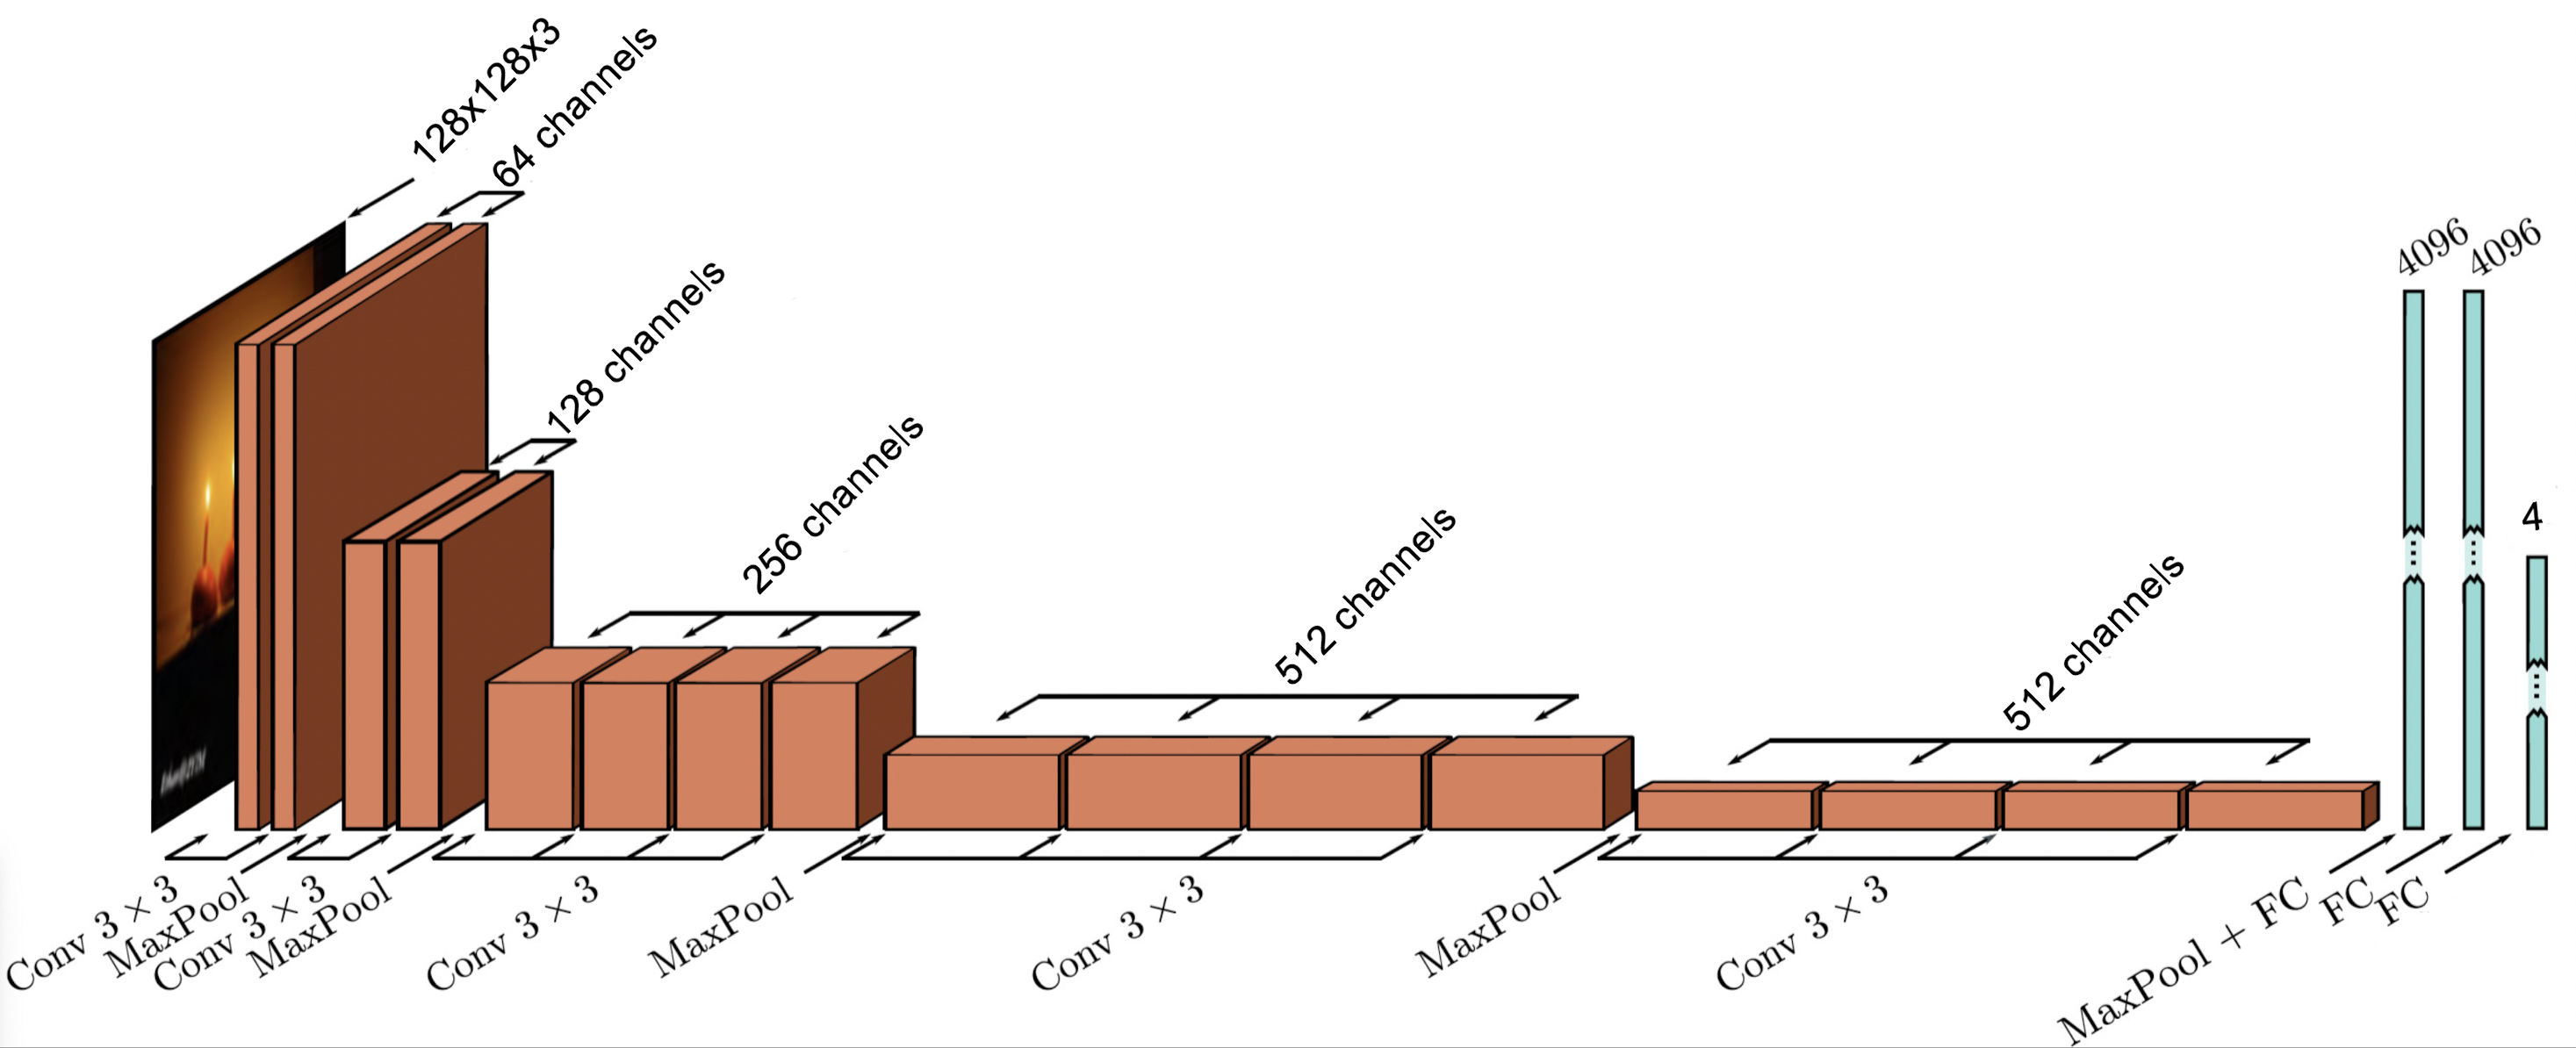
\includegraphics[width=1.1\textwidth]{vgg_arc.png}
    \end{center}
    
    Number of parameters: $65070916$\\
    Dropout rate: $0.5$
\end{frame}

\begin{frame}
    \frametitle{Setup Differences}
    \hspace*{-0.7cm}
    \begin{tabular}{|c|c|c|c|c|}
        \hline
        \textbf{Model} & \textbf{Data augmentation} &\textbf{LR Scheduler} & \textbf{Activation} & \textbf{L2 reg.} \\
        \hline
        CustomCNN & Yes & Yes & $Mish$ & Yes \\
        AlexNet & No & Yes & $ReLU$ & Yes \\
        VGG16 & No & No & $ReLU$ & No \\
        VIT & Yes & Yes & $Mish$ & Yes \\
        \hline
    \end{tabular}\\
    \vspace{0.5cm}
    \begin{cbox}
        \begin{itemize}
            \item All the other hyperparameters and settings are the same for all models(batch size, optimizer, epochs, etc)
            \item Note that the \textbf{CustomCNN} is the one with less parameters ($3,001,156$) while \textbf{VGG16} is the one with more parameters($65,070,916$)
            \item \textbf{VGG16} is also the one with the highest dropout rate ($0.5$)
        \end{itemize}
    \end{cbox}
\end{frame}

\begin{frame}
    \frametitle{Performance Assessment}
    \begin{itemize}
        \item \textbf{Loss function}: Cross-entropy loss $L(y, \hat{y}) = -\sum_{i} y_i \log(\hat{y}_i)$
        \item \textbf{Accuracy}: Number of correct predictions divided by the total number of predictions
        \item \textbf{Confidence}: Given by the Softmax function applied to the net output $S(x_i) = \frac{e^{x_i}}{\sum_{j} e^{x_j}}$
    \end{itemize}

\end{frame}

\begin{frame}
    \frametitle{Training Loss and Accuracy for AlexNet}
    \begin{center}
        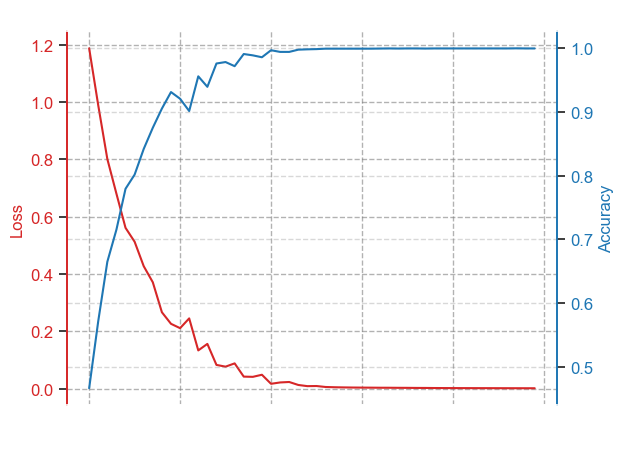
\includegraphics[width=0.65\textwidth]{alex_loss_acc.png}
    \end{center}

    \small{
    \begin{cbox}
        \begin{itemize}
            \item Final training loss: $1.2\cdot 10^{-3}$
            \item Final training accuracy: $99.9\%$
        \end{itemize}
    \end{cbox}
    }
\end{frame}

\begin{frame}
    \frametitle{Confidence and Test Accuracy for AlexNet}
    \begin{center}
        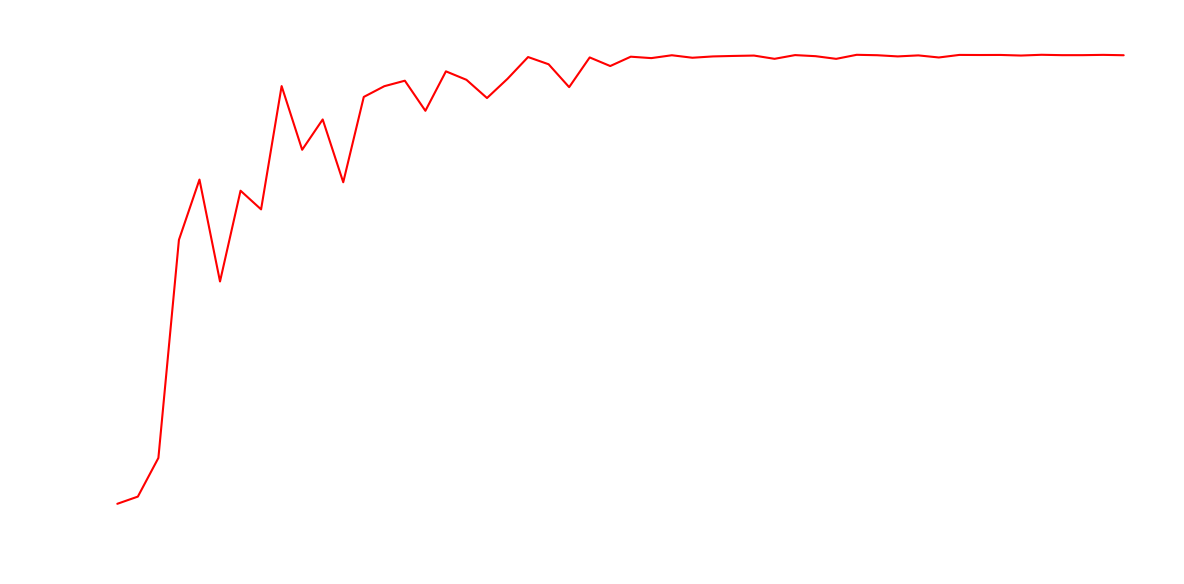
\includegraphics[width=0.65\textwidth]{ale_conf.png}
    \end{center}

    \small{
    \begin{cbox}
        \begin{itemize}
            \item Final training confidence: $99.9\%$
            \item Final test confidence: $96.5\%$
            \item \red{Final test accuracy: $90\%$}
        \end{itemize}
    \end{cbox}
    }
\end{frame}

\begin{frame}
    \frametitle{Training Loss and Accuracy for VGG16}
    \begin{center}
        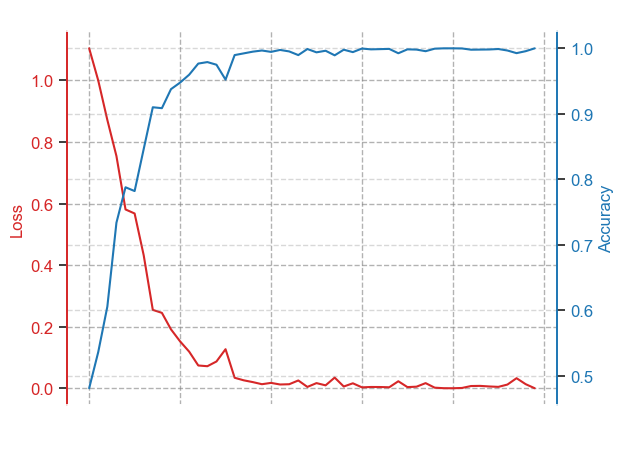
\includegraphics[width=0.65\textwidth]{vgg.png}
    \end{center}

    \small{
    \begin{cbox}
        \begin{itemize}
            \item Final training loss: $8.9\cdot 10^{-6}$
            \item Final training accuracy: $99.9\%$
        \end{itemize}
    \end{cbox}
    }
\end{frame}

\begin{frame}
    \frametitle{Confidence and Test Accuracy for VGG16}
    \begin{center}
        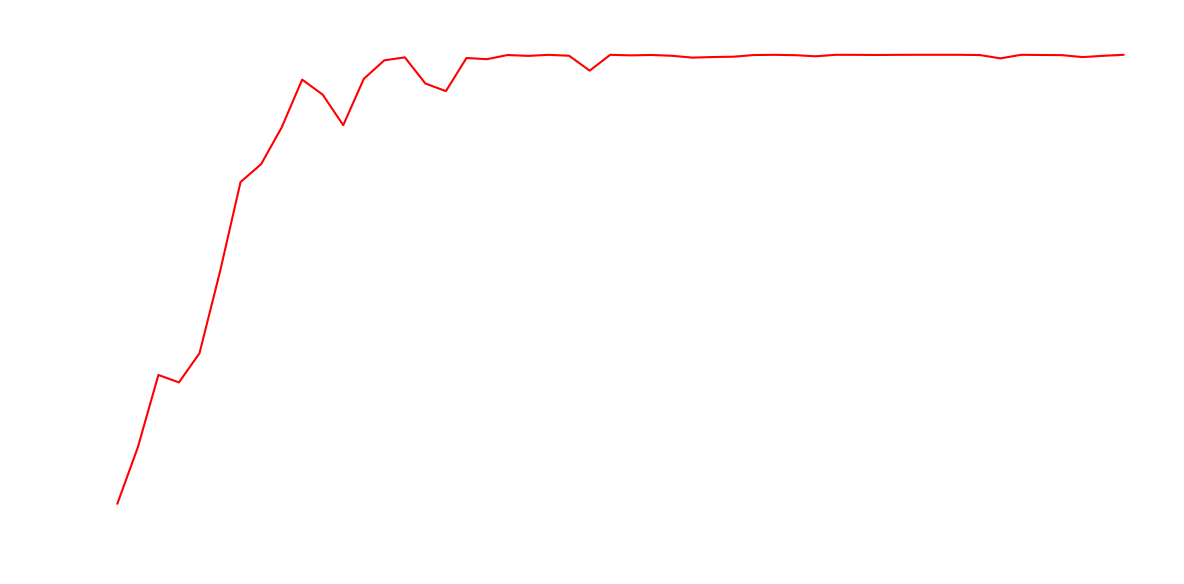
\includegraphics[width=0.65\textwidth]{conf_vgg.png}
    \end{center}

    \small{
    \begin{cbox}
        \begin{itemize}
            \item Final training confidence: $100\%$
            \item Final test confidence: $98\%$
            \item \red{Final test accuracy: $95\%$}
        \end{itemize}
    \end{cbox}
    }
\end{frame}

\begin{frame}
    \frametitle{Training Performance Comparison}
    \centering
    \begin{tabular}{|c|c|c|c|}
        \hline
        \textbf{Model} & \textbf{Loss} & \textbf{Accuracy} & \textbf{Confidence} \\
        \hline
        CustomCNN & $1.4 \cdot 10^{-3}$ & 0.99 & 100\% \\
        AlexNet & $1.2 \cdot 10^{-3}$ & 0.99 & 99.9\% \\
        VGG16 & $8.9 \cdot 10^{-6}$ & 0.99 & 100\% \\
        VIT & 0.27 & 0.90 & 96.1\% \\
        \hline
    \end{tabular}\\
    \begin{cbox}
        Note that these are the values reached during the last epoch.
    \end{cbox}
\end{frame}

\begin{frame}
    \frametitle{Focus on Accuracy}
    \begin{center}
        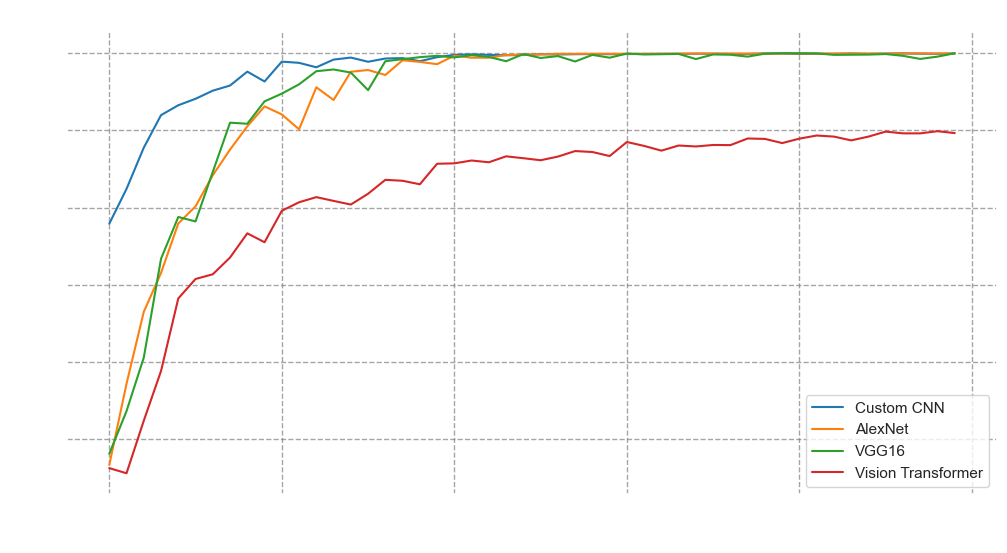
\includegraphics[width=1\textwidth]{accuracy_compared.png}
    \end{center}
\end{frame}

\begin{frame}
    \frametitle{Test Performance Comparison}
    \centering
    \begin{tabular}{|c|c|c|}
        \hline
        \textbf{Model} & \textbf{Accuracy} & \textbf{Confidence} \\
        \hline
        CustomCNN & 0.99 & 100\% \\
        AlexNet & 0.90 & 96.5\% \\
        VGG16 & 0.95 & 98.0\% \\
        VIT & 0.88 & 93.3\% \\
        \hline
    \end{tabular}\\

\end{frame}

\begin{frame}
    \frametitle{Visualizing the first layer filters, CustomCNN}
    \begin{center}
        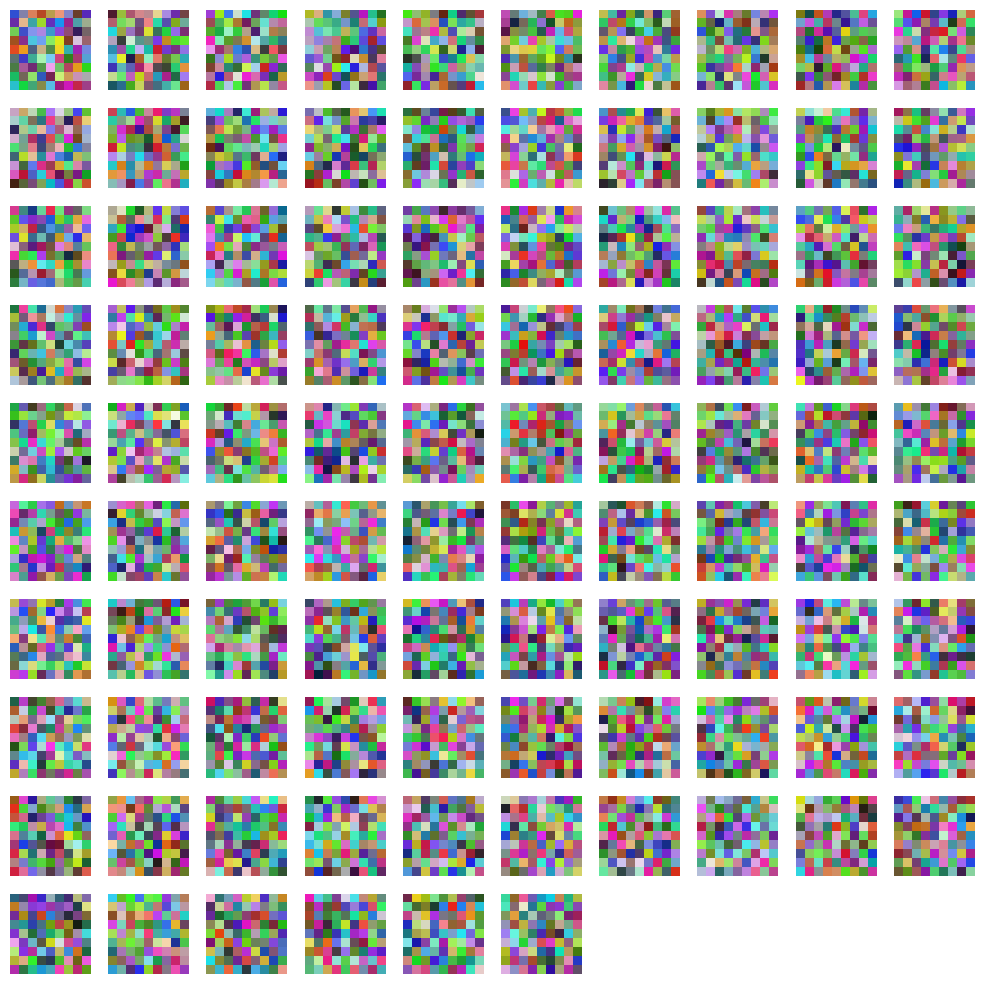
\includegraphics[width=0.7\textwidth]{cnn_conv.png}
    \end{center}
\end{frame}

\begin{frame}
    \frametitle{Visualizing the first layer filters, AlexNet}
    \begin{center}
        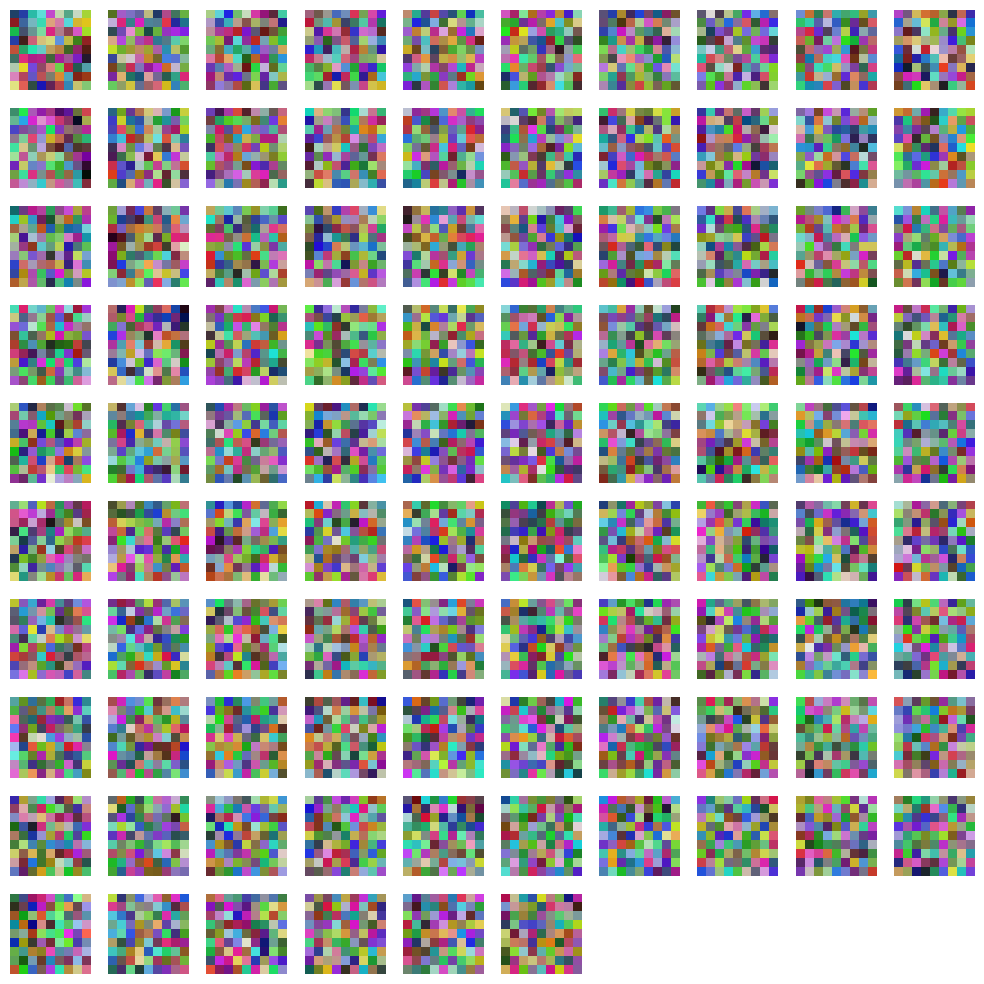
\includegraphics[width=0.7\textwidth]{alex_conv.png}
    \end{center}
\end{frame}

\begin{frame}
    \frametitle{Visualizing the first layer filters, VGG16}
    \begin{center}
        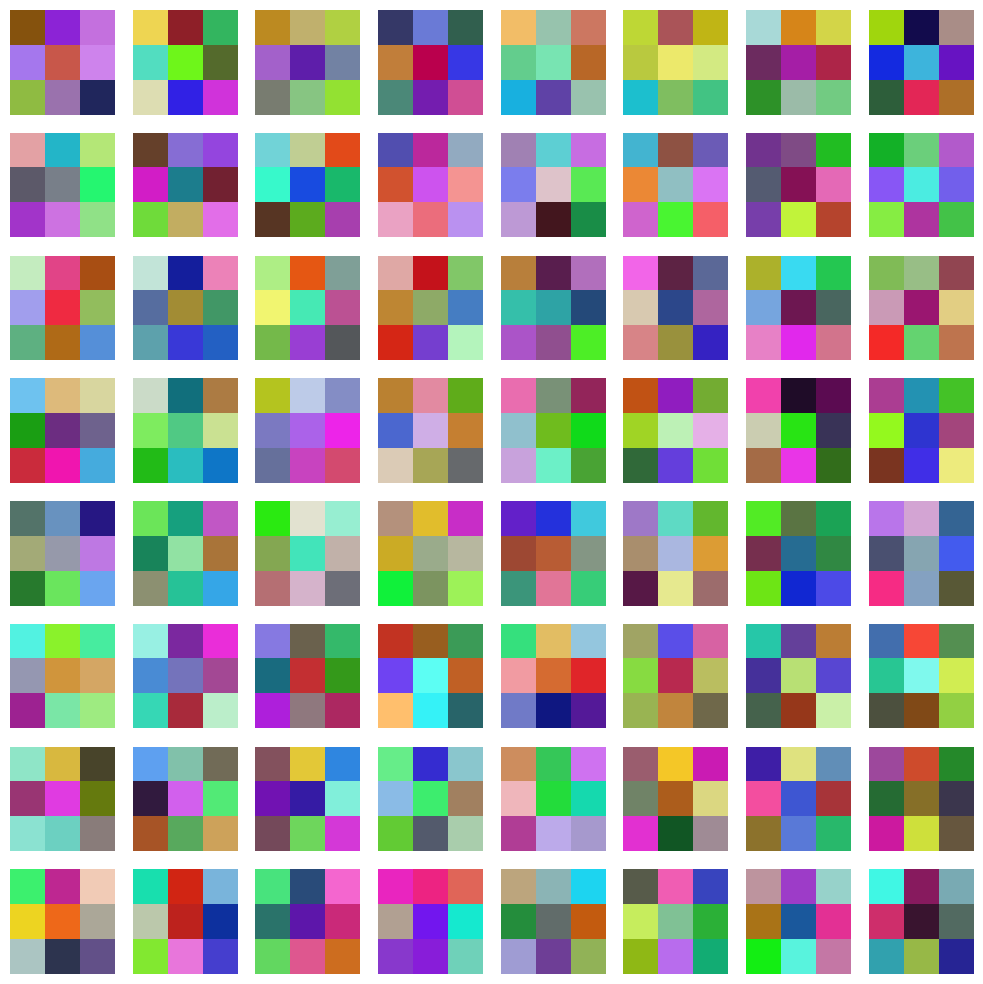
\includegraphics[width=0.7\textwidth]{vgg_conv.png}
    \end{center}
\end{frame}

\end{document}
